%Known to compile with pdflatex with texlive installation
%Known to NOT compile with pdftex with texlive installation
%
%For use of the tools exploited in this paper, see
%  http://wiki.datakurator.net/web/FP-Akka_User_Documentation
%  wiki page based on 1.5.2 Release of FP-Akka
%  That wiki page has permalink http://wiki.datakurator.net/w/index.php?title=FP-Akka_User_Documentation&oldid=438 but any later release of the FP-Akka_User_Documentation should also work.

%postprocess.jar produced with  wget https://sourceforge.net/projects/filteredpush/files/fp-postprocess/releases/fp-postprocess-RELEASE-1.1.6.zip
%   and unzipping in this directory
%workfloswtarter.jar produced with  wget https://sourceforge.net/projects/filteredpush/files/FP-Akka/releases/FP-Akka-1.5.2-workflowstarter.jar


\documentclass{article}
\usepackage[utf8]{inputenc}
%\usepackage[english]{babel}
\usepackage{currfile}
\usepackage{natbib}
%\usepackage{cite}
\bibliographystyle{plainnat}
%\bibliographystyle{alpha}
\usepackage[document]{ragged2e} %ragged right
\setlength{\parskip}{10pt plus 1pt minus 1pt}
\usepackage{fullpage} %1 in margin
\usepackage{graphicx}
%\usepackage{calc}
\usepackage{listings}
\usepackage{lineno}
\usepackage{rotating}
%\usepackage{makecell}
%\usepackage{tabularx}
\usepackage{longtable}
\usepackage{tablefootnote}
\linenumbers

%tablestuff
\newcommand{\tablebar}{\hspace{3pt}\textbar\hspace{3pt}}
%\usepackage[dvipdf]{xcolor,colortbl}
%\usepackage[dvipdf]{color}
\usepackage[svgnames]{xcolor}
\usepackage{colortbl}
\usepackage{getfiledate}
%\newcommand{\editor}{ram, pjm}  %signify manuscript editor identi
\newcommand{\editor}{ram}  %signify manuscript editor identi
\newcommand{\version}{{\currfilebase .tex} {edited by \editor }}
%\newcommand{\filedate}{\getfiledate{\currfilebase .tex}}

\usepackage{fancyhdr}
\pagestyle{fancyplain}
\lfoot[\fancyplain{\version}{\version}] {\fancyplain{\version}{\version}}
\cfoot[\fancyplain{\thepage}{\thepage}] {\fancyplain{\thepage}{\thepage}}
%\rfoot[\fancyplain{\filedate}{\filedate}] {\fancyplain{\filedate}{\filedate}} %puts where getfiledate wants it, below footer
%\setlength{\headheight}{24pt}
\setlength{\headheight}{18pt}

\usepackage{hyperref}
\usepackage[titletoc]{appendix}

\begin{document}
\title{Flags are not enough: A friendly spreadsheet user interface for Quality Control of occurrence data.}
\author{Morris, Morris, Lowery, Song}
\begin{abstract}
An analytical consumer of large natural science collections data sets may be satisfied with data quality reports that allow inclusion or exclusion of subsets of the data from analysis based on some fitness for purpose criteria.  A data curator, however, will much more likely need more information concerning the provenance of data quality assertions in order to rationally act on those assertions to improve the quality of their data set, by some data quality criteria and measures.  We describe a friendly, spreadsheet-based data quality report produced by tools developed by the FilteredPush and Kurator projects. The structure of the report is influenced by the needs of data curators and data users.  The report is in the form of a multi-sheet spreadsheet containing a summary sheet and sheets reporting the details of data quality for particular conceptual operations on the data (e.g. georeference validation).  The detailed report sheets include flags to assert the status of each row of data, original data and proposed corrections. Also included are a list of external sources that were consulted in the evaluation of each row, and a human readable comment that reflects a provenance trace through the internal logical steps taken by the data quality software.  
%We also discuss expectation management of consumers of data quality reports in the light of data quality assertions in those reports reflecting defects in the data, the software, or consulted services.
%ram: we only do this briefly at the end, so I would leave this out
\end{abstract}
\section{Introduction}
Data about occurrences of organisms at particular places and times support many scientific endeavors ranging from environmental studies to evolutionary hypotheses to climate change studies. 
Both users and managers of such data have a distinct need to understand the fitness of such data for the use to which they will put it. 
These needs arise both about specimens preserved in natural science collections as vouchers for the occurrence, or unvouchered human or machine observations.
Users and data managers are also concerned with the ease, reliability, and repeatability with which that data can be accessed and aggregated with related data.  
These concerns can all be discussed under the rubric of data Quality Control (QC), a discipline historically focused on manufacturing,  which arguably originated with the 1922 publication by Radford of “The Control of Quality in Manufacturing” \citep{radford_control_1922}. Radford's preface relates:
\begin{quotation}
  In the factory, quality is a costly thing to neglect, yet it is the usual experience to find a disproportionate emphasis placed upon quantity of output, in the effort to effect economies. Often, this is not so much due to lack of proper intent as it is to the failure to realize what the quality approach means. […] if quality is under positive and continuous control, increase of output follows as a by-product advantage.
\end{quotation}
In the first few decades of natural science collection digitization the emphasis was on careful, rich transcription of all of the details of paper records associated with specimens.  In the 1990s, recognition arose that specimens were entering collections at a faster rate than digital records could be created with such detail and high data quality. Hence, particularly in recent large scale digitization (e.g. \citep{ADBC} and \citep{Haston2012}), focus has shifted to rapid transcription of fewer data elements, with an emphasis on making dark data accessible \citep{ZooKeys209,Smith2012}.
%%%Thus attention often turns first to the creation of adequate minimal electronic records from paper records for some research uses of the data and ready electronic discovery of the paper records for other research uses.  
%\textbf{PJM: RAM made citation of Haston2012 less specific, and took out reference to funding. But it is still a confusing final sentence}
%%% Mumble here about workflow?
  \section{Shifting historical foci of concern}
As Chapman pointed out over 10 years ago \citep{chapman_principles_2005}, Quality Control of biotic occurrence data shares many QC concerns with those of other science disciplines and those of manufacturing. 
In the context mentioned above, we could recast Radford's preface as:
\begin{quotation}
  In the natural science collection, data quality is a costly thing to neglect, yet it is the usual experience to find a disproportionate emphasis placed upon quantity of output, in the effort to effect economies.
\end{quotation}

  This formulation evokes Shewhart's Plan-Do-Check-Act model \citep{shewhart_statistical_1939}, wherein a QC application performs checks and the resulting outcome is a basis for Act. A more modern, explicitly {\em data} quality control model, would phrase this as the Define-Measure-Analyze-Improve meme in \citep{Wang1998}.  
%{Depending on when Allan submits a paper with analysis of FP-Akka, should perhaps cite here, but agreed not yet...ram}

  Albeit with some resistence \citep{ShetlerDemyth1974}, natural science collections digitization began in earnest in the 1970s (e.g. with SELGEM \citep{SELGEM1971}; CITE NSF reports), with a prescient vision (CITE, malacology standard?) of the power for research of data exchanged and aggregated across all collections. Chronicaling the history of computerization at the Berkeley Museum of Vertrate Zoology, Sunderland \citep{Sunderland2013150} relates that institutions had already noticed that the costs associated with mainframe computing didn't justify systems devoted only to cataloging specimens. Computers would also have to support the storage and discovery of scientific knowledge as well.  

In the 1980s, there was widespread recognition that this long term vision of data interchange needed common understanding of concepts and vocabularies across collections and documents.  Influential models for common concepts emerged in the late 1980s and early 1990s, in particular the ASC model \citep{ASC1992}, and early versions of HISPID \citep{HISPID5} and ABCD \citep{ABCD2015}.  In 1985, the Taxonomic Databases Working Group (TDWG) emerged as a forum for global standardization efforts in the domain \citep{tdwg_tdwg_2007}. (Although the acronym remains in wide use, the organization is a body now named Biodiversity Information Standards (TDWG)).  An emphasis of TDWG in the 1980s and 1990s was the development of controlled vocabularies to promote the exchange and integration of taxonomic data.
  
%Not wholly correctly,
Somewhat inaccurately,
we could characterize this phase of the development to the digitization of natural science collections data as Plan-Do. That is, plan out the designs for information systems and controlled vocabularies for data capture, and do, build them and populate them with data.   An emphasis in the 1990s was to design information systems that limited the ability of data entry personnel to make mistakes \citep{MorrisP2005}.  
Networks developed first for distributed query (e.g. FishGopher \citep[see][p.92]{wiley_biodiversity_2004}, MaNIS \citep{BI7, manishome_2015}, VertNet \citep{VertNetAbout}, HerpNET \citep{herpnet_2016}, FishNet \citep{fishnet_2016}, ORNIS \citep{ornis_2016}\footnote{The data portals of ORNIS, MaNIS, FishNet, and HerpNET have recently been merged with that of VertNet, although the underlying collaborations generally remain intact.}, BioCase \citep{BioCase_2015}).
These were followed quickly by networks and other tools for data aggregation of natural science collections data (OBIS \citep{OBIS2011}, GBIF \citep{GBIF2015},  iDigBio \citep{iDigBio2015}), along with shifts in the emphasis in digitization strategies from rich data capture to rapid data capture from bulk data sources (e.g. transcription from handwritten ledgers).
Consequent data growth and availability led to an increasing recognition of data quality issues (e.g. \citep{Frey200616}).
At the same time introduction of networks of unvouchered observational data (e.g. eBird  \citep{sullivan_ebird:_2009} and \citep{Ahumada2703}) led to even more rapid data growth. 
With these devlopments has come the understanding that fitness for reuse demands more and more emphasis on data quality control (e.g. \citep{chapman_principles_2005}). Along with classical taxonomic uses, species occurrence data is valuable for research questions related to global change, ecological studies, and agricultural applications (e.g. \citep{brooke_why_2000,Graham2004497}.)  In the face of these changes, the community has shifted further towards Check-Act, checking data quality and acting to improve it (e.g. \citep{eBirdQC}.)  

TDWG collaborates with the Global Biodiversity Information Facility (GBIF), an international treaty-based organization that provides an open data infrastructure funded by signatory governments. 
At this writing, GBIF's data portal aggregates almost 625 million occurrence records of over 1.6 million species. These records are aggregated and indexed over 29,000 datasets published by 821 data publishers worldwide. GBIF produces software tools and components, notably several for producing and managing Darwin Core Archives (see \citep{GBIF_DWCA}), that are capable of publishing occurrence data coded to TDWG's Darwin Core (DwC) controlled vocabulary \citep{wieczorek_darwin_2012, tdwg_darwin_2015}. 
These document both specimens and unvouchered observations. The latter are growing faster in number. For example, as of October 11, 2016, GBIF serves nearly four times as many observation records as specimen records, compared to a factor of three a year earlier.

Following common conventions, if a vocabulary term is defined in DwC we will preface it with “dwc:”. 
\section{Assertions vs “facts”}
For over a century, practicing taxonomists have agreed that classification and description of biotic occurrences often involves professional opinions that are subject to revision and dispute:
\begin{quotation}
``There can be no precise criterion of species. `Species' is a human concept as much as `genus,' and of the same sort.'' (\citep{lutz_variation_1908} p.7.)
\end{quotation}

For this and other reasons, many artifacts of taxonomic data Quality Control are themselves represented as assertions about fitness for use, not necessarily affirmation or denial of factual correctness. Simple cases are the logical correlation between several data attributes sometimes assembled by the FilteredPush (FP) \citep{filteredpushWeb_2016} project's workflows. For example, in cases where we have access to services giving biographical data of collectors (e.g., the machine-accessible service Harvard Index of Botanists \citep{harvard_university_herbaria_&_libraries_index_2013}, the workflow components may query such services to examine the lifespan of the names of the collectors named in the “dwc:recordedBy” attribute. If the collection date falls outside these lifespans, the workflow can only assert that the biographical and collection data cannot simultaneously be correct. This leaves it to the workflow user to decide which, if either, should be deemed correct and what to do about this. More technical details of the FP workflow components are to be found in \citep{song_towards_2014}.  

In this paper, we are principally concerned with a friendly spreadsheet-based user interface aimed at helping data curators and other users evaluate the fitness for use of FilteredPush QC assertions generated by the Java-based application that we call \emph{FP-Akka}. 
%\textbf{Generality of applicability. Where does sentence below belong?} 
Most of the FP-Akka components assume that the input occurrence data are coded with attributes named, except for case sensitivity,  by the Darwin Core term names.



\section{FP-Akka Architecture}

\begin{figure}[b!]


%\includegraphics[width=\textwidth]{Fig1.png}
%\includegraphics[width=\textwidth]{FP-Akka-architecture_diagramv2.png}
%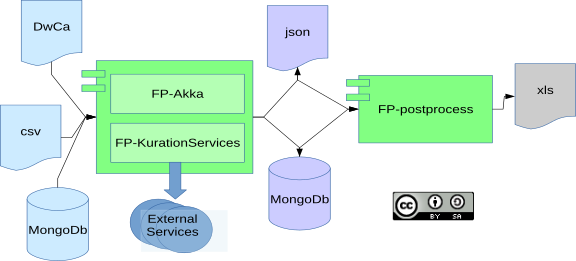
\includegraphics[width=\textwidth]{Architecturev4.png}
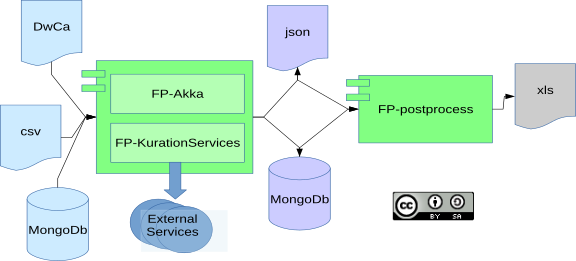
\includegraphics[width=4in]{Architecturev4.png}
\caption{FP-Akka Architecture}
% ram: need to define MongoDB and xls.  Need to put FP-Akka-workflowstarter label in the diagram**  FP-Akka-workflow starter can take DarwinCore archives, flat DarwinCore in a CSV file, or flat DarwinCore records as JSON loaded from a MongoDB datastore, can run data quality control processes on them, using data quality logic in the FP-KurationServices library, and write output as richly structured data in JSON to the file system or into MongoDB.  A key challenge discussed in this paper is rendering this rich structured output in a human readable form that can be acted upon by data curators.  The FP-postprocess component is responsible for this rendering, converting the JSON into a spreadsheet.}
\label{fig:architecture}
\end{figure}
Figure \ref{fig:architecture} describes the architecture of FP-Akka. The platform takes its name from its use of  the open source Akka platform for high performance, asynchronous, distributed applications \citep{akka_akka_2015}. Currently, two artifacts are provided for users to run. The first, \emph{FP-Akka-workflowstarter jar}, is a Java application that takes various flat DarwinCore inputs, and creates intermediate JSON (JavaScript Object Notation) \citep{ecmaJSON} output. The second, the \emph{FP-Akka postprocessor}  \citep{FP_postprocess} creates human readable spreadsheets from the intermediate JSON.  The FP-Akka-workflowstarter application itself includes the \emph{FP-Akka} component  that describes a data flow workflow paralellized with the Akka framework, and the FP-KurationServices component, which contains the internal implementations of domain specific data validation actors. The latter invokes a range of external services provided by authoritative sources in the community.   The code base of FP-Akka seeks to separate concerns of dataflow management, domain data quality business logic, web service invocation, and presentation to end users.  The FP-KurationServices code had its origins in the Kepler-Kuration module \citep{dou_kurator_2012, dou_scientific_2011}, which presented a proof of concept of a data quality control workflow written within the Kepler workflow environment.   Key elements of the metadata concerning data quality assertions by the code, the Curation Status, the Curation Comment, and the Services Consulted, have been retained from the Kepler-Kuration work. These represent an interface between the internal business logic of a data quality control actor, and the flow of data and metadata in the workflow. 
They also represent the key elements we have identified for clustering and interpretation of data quality assertions by end users.  The curation status is the key sorting element for analytical uses (i.e., does this record meet inclusion/exclusion criteria based on a test of fitness for some purpose).  The services consulted and the curation comment provide critical provenance information about each data quality assertion that allows a data curator to assess what actions, if any, to take on the data elements involved in that assertion.  
Since the time of the Kepler-Kuration implementation, a number of components have changed. These include the workflow framework itself, particular workflows and presentation mechanisms. Also, the internal quality control logic of the actors has been reworked. However, the \emph{interface} for presentation of the assertions made by the quality control code to downstream consumers (e.g plugins to Symbiota and other specimen management systems, as well as the new postprocessor that is the subject of this paper) has remained unchanged. That interface remains described by the aforementioned intermediate JSON.

\section{Validators}
FP-Akka presently supports five principal data quality actors which are put together with input and output components for the purpose of deriving QC assertions about taxon occurrence data.  
These actors, which we call ``validators,'' are the ScientificNameValidator, the EventDateValidator, the DateValidator
%\footnote{explain date stuff},
\footnote{See, e.g. http://rs.tdwg.org/dwc/terms/\#Event for date forms available to the EventDateValidator and http://rs.tdwg.org/dwc/terms/\#Taxon for some data available to the ScientificNameValidator.}
 the GeoReferenceValidator, and the BasisOfRecordValidator.   
%These actors may have unique or multiple  Darwin Core attributes in appropriately coded occurrence data, e.g. Darwin Core Archives 
The validators act on appropriately coded occurrence data, e.g. Darwin Core Archives 
(\citep{robertson_dwca_2015}) 
 or simple comma separated values (CSV \citep{ietf4180})-coded text files.
For example, the ScientificNameValidator can make QC assertions about dwc:scientificName and about the authorship of a name (dwc:scientificNameAuthor).  The actors in FP-Akka consist almost entirely of code that manages the flow of data and data quality assertions through the workflow.  All of the business logic of data quality control is separated into classes in the FP-KurationServices module.   The FP-Akka actors are composed into workflows.  Three workflows are in current production use in FP-Akka. The first is the standalone \emph{DwCa workflow} that takes DarwinCore data in the form of CSV files or DarwinCore archives and passes it through 
%the ScientificNameValidator, DateValidator, GeoreferenceValidator, and BasisOfRecordValidator 
the validator, and then writes the intermediate JSON output to a file. 

The second DwCa workflow is illustrated in Section \ref{dwcaworkflowsec}.  It is intended to allow users to run analyses on their own data sets.  A similar workflow is embedded in FilteredPush network nodes as an analytical capability (NEED A GOOD REF).  It is identical to the standalone DwCa workflow except for data loading and writing actors that interact with MongoDB \citep{mongodb_inc_mongodb_2015} instead of the filesystem. 

The third workflow consists of a CSV reader, the ScientificNameValidator and a CSV writer. 
It is intended for checking taxonomic authority files in collection databases. 
This workflow takes a CSV dump from a natural science collection database taxonomic authority file comprising the primary key from the table, the scientific name, and the scientific name authorship. 
The workflow output retains the primary key value, and adds values for corrected scientific name and scientific name authorship if provided by a name authority. If the name authority offers a globally unique id (GUID) for \emph{its} record, that GUID is added to the output as provenance.
Also in the output are the original values for the scientific name and scientific name authorship, as well as the curation status. Added provenance called ``Comment'' is provided in the FP-Akka JSON output but labeled as ``Provenance'' in the spreadsheet models, as illustrated in Table \ref{ExampleQCAssertions}.  Each addition is rendered as a column in the output CSV file. 
This format provides a very effective tool for database managers, since a text pattern matching utility such as \emph{grep} \citep{wikiGrep}
can isolate lines that contain a particular QC assertion.  Each line contains the input value of the database primary key along with an assertion of a GUID found for the matched name in the specified authority. Hence, regular expression tools can readily convert a set of lines into SQL update statements that can be fired against the database to add the GUID to validated records (identfied by their database primary key).  For example, the output line: 
\begin{quotation}\noindent\texttt{``62740'',``Scientific Name Authorship was empty'',``changed to: Walckenaer, 1805''}\end{quotation}
from Table \ref{ExampleQCAssertions} is easily transformed into the SQL query 
\begin{quotation}\noindent\texttt{``update taxon set SciName = `Latrodectus Walckenaer, 1805' where taxonid = 62740''.}\end{quotation}
Likewise grep can identify particular kinds of problems found in the dataset and the corresponding rows can be put into a spreadsheet and sent, as a trackable unit of work, to collection management staff for evaluation and correction of the relevant database records.

%\begin{figure}[h]
%\caption{YesWorkfow diagram of the DwCa workflow.  **need caption text**}
%\label{fig:dwcaworkflow}
%\end{figure}

Some Darwin Core attributes have both an atomic form comprising several components and a federated form conforming to some data standard or authority.  For example a record set may have values for the year, month and day of the collection event, and also a value for dwc:eventDate comprising a date string compliant to the DwC-recommended ISO 8601 date standard \citep{iso_iso_2004}. 
The FP-Akka DateValidator can compare an ISO 8601 date constructed from the three atomic fields to that given by (or missing from) dwc:eventDate.

Each validator produces its assertions as one of five outcomes along with provenance information, i.e., information about how and why the validator came to make those assertions. Of particular provenance interest is the authority for the outcome, including well-known authority servers and caches that a particular configuration may support.  For example, a user who knows that the  input  comprises entirely plant data can arrange to consult specific plant-centric taxonomic name authorities such as the International Plant Names Index (IPNI) \citep{ipni_international_2012}. 
%DROPPED BY RAM in QC16 textbf{\We should drop this bit about the list of botanists or move it elsewhere, authority is specified only for scientific name validation, and has no linkage to event date validation, the list of botanists also contains people who have worked on fungi and non-vascular plants, so the discussion is much more complex than just ipni=botanist list ok. Such a user can put credence on the biographical data found in the Harvard List of Botanists used to validate collection event dates as mentioned earlier.  By default, the List of Botanists is always consulted, so it always important for event date validation provenance to clearly remark that the Harvard List was consulted and what assertions were deduced therefrom.  We are unaware of biographical services suitable for collectors of other groups, nor any service more general than the Botanists List. [PAUL SAYS: Unaware isn't right, we know of library data on authors, Kew has relevant services, etc.]}
Specialist knowlege of scope of the external resources consulted is important.  IPNI is an authority on the nomenclature of vascular plants, but currently does not have strong coverage of non-vascular plants, or fungi (which are also covered by the botanical code of nomenclature, ICNafp \citep{ICNafp2012}.  Under the current architecture of FP-Akka, a holder of a botanical data set would have to make an informed choice about selection of IPNI or IndexFungorum (IF) \citep{IF_2015} based on their knowlege of the taxonomic scope of their data.  
%\pagebreak
\section{Outcome Values}
\begin{table} %[!h]
\setlength\arrayrulewidth{2pt}
\small
\begin{tabular}{ |p{1.0in}|p{1in}|p{0.75in}|p{0.75in}| }
 \hline
%\multicolumn{4}{c}{Table 1 FP-Akka Outcomes}\\ \hline
\textbf{Validation Outcome} &\textbf{Assertion about object validated} &\textbf{Workflow outcome label} &\textbf{Spreadsheet cell color}\\ \hline
CORRECT & Nothing found wrong & \cellcolor{LightGreen}no change needed; looks good to us&\cellcolor{LightGreen}Green \\ \hline
CURATED &Proposed change&\cellcolor{yellow}we have proposed this change &\cellcolor{yellow}Yellow \\ \hline
FILLED\_IN & Proposal for a missing attribute &\cellcolor{LightGoldenrod}no value present; we have proposed one &\cellcolor{LightGoldenrod}Mustard\\ \hline
UNABLE\_\newline DETERMINE\_\newline VALIDITY &Can’t tell whether value is valid (generally, preconditions for validation were not met).&\cellcolor{gray}don't know&\cellcolor{gray}Gray \\ \hline
UNABLE\_\newline CURATE &Value is not validated but workflow can’t suggest a change&\cellcolor{red}there seems to be a problem, but we don't know how to solve it&\cellcolor{red}Red \\ \hline
\end{tabular}
%{FP-Akka Outcomes}% \tablefootnote{See Table \ref{ExampleQCAssertions} }} %\ref{ExampleQCAssertions} } 
\caption{FP-Akka Outcomes}% %{FP-Akka Outcomes \footnotemark\footnotetext{See foo} } 
\label{FPAkkaOutcomes}
\end{table}
%\end{document}
 %Table of outcomes
The data quality control logic (in FP-KurationServices classes as shown in Figure \ref{fig:architecture}) returns a validation state (for the evaluation of a particular set of fields for a particular record), with one of five values.  These are passed on to the intermediate JSON as one of five strings (``Validation Outcome'' column in Table \ref{FPAkkaOutcomes}).  These values are “CORRECT”, “FILLED\_IN”, “CURATED”, “UNABLE\_DETERMINE\_VALIDITY”, and “UNABLE\_CURATE”
\footnote{See also Table \ref{ExampleQCAssertions} for examples derived from the postprocessor.}.
An assertion that a value is correct is a claim that the data quality control logic found no inconsistency between the data presented and any oracles that it consulted.  
This may mean that the data was validated, as in the case of the ScientificNameValidator finding a single exact match for a scientific name string and authorship in IPNI, and being able to assert IPNI's LSID for the matching IPNI nomenclatural record.
CORRECT may also mean that the data was merely consistent, as in the case of the collecting event DateValidator asserting that a particular collection date in dwc:eventDate falls within the lifespan of the collector in dwc:recordedBy as asserted by a biographical record for a person who's name matches the string found in dwc:recordedBy.  The collecting event date could still be off by days or months or years, but the data quality code was not able to detect a problem.

An assertion that the outcome was FILLED\_IN represents an orthogonal concern that we have not untangled in the FP-Akka development (but are addressing in ongoing Kurator project development \citep{Kurator_wiki_2016}).  That is, a dwc:eventDate may have been empty, but a dwc:day, dwc:month, and dwc:year may have allowed us to construct an event date and compare it with any known collection dates for the collector.  An assertion about the comparison of the dwc:eventDate with the collector's lifespan is an orthogonal concern to our having filled in dwc:eventDate from related data elements.  This orthogonality highlights a defect in FP-Akka in that it can only present a single outcome for a given data record. 

An assertion that the outcome was CURATED is that the data quality code has found an inconsistency between the data and an oracle, and is proposing a correction based on the value from the oracle.  If we have been careful in the interpretation of results returned from external authoritative services, and if those services themselves are accurate, then this proposed correction is probably reasonable.  Proposed corrections of scientific names have posed the greatest challenge here.  Scientific name authorities can vary in quality, and if selected, can return values that knowledgeable users consider to be incorrect. 


An assertion that the outcome was UNABLE\_DETERMINE\_VALIDITY can result from a precondition for the evaluation not being met. 
Examples include scientific name validation for a record that lacks a dwc:scientificName and dwc:scientificNameAuthorship, or an orthogonal concern that the execution hasn't yet untangled, or a failure of an external service to respond to a query from the data quality code.

An assertion that the outcome was UNABLE\_CURATE corresponds to the sense of ``SolveWithMoreData'' in \citep{morris_semantic_2013}.  It is an assertion that the data quality control code found a problem, but was not able to propose a solution to that problem.  
A composite record that contains textual locality information that describes one place on the surface of the Earth but a georeference for a different locality in a different country would produce this outcome.
The georeference would be identified as inconsistent with the polygon for dwc:country, and if no transposition or sign change for the coordinates placed them near (e.g. within 20 km) of a georeference for the textual locality data as asserted by the geolocate service, FP-Akka would mark the outcome as UNABLE\_CURATE.  
A human will need to evaluate this record and determine if the problem lies in the textual locality data, in the georeference, or in some other circumstance.
An example of the latter is in the ``Bernardo Assertion'' in \citep{morris_semantic_2013}), where identifications from three specimens were mis-transcribed by assigning locality data from three other specimens.

Presenting these outcome values to end users as short phrases posed a challenge.
We initially presented them as icons accompanied by color coding of cells in a result spreadsheet. (See discussion at \citep{FPWiki_ResultTypes}.)  Following repeated user feedback, we changed these to the text values, and then to brief human readable phrases shown in the ``Outcome'' 
column in Table \ref{ExampleQCAssertions}. %\ref{FPAkkaOutcomes})
% which we have tuned from repeated user feedback to the current values.   
These labels capture the gist of the outcome (e.g. ``CORRECT'' carries  ``no change needed; looks good to us'', where the ``good to us'' has the implication 
that the result may not be correct.)

The entries in Table \ref{ExampleQCAssertions} were derived from actual data produced by FP-Akka applied to several specimen records at the Harvard Museum of Comparative Zoology.
Curation status outcome phrases like these may be adequate for an analytical user of a large data set to include/exclude records that fit particular data quality criteria.  They are, however, inadequate for a data curator assessing whether to apply the change proposed along with an outcome of CURATED to the database of record, or whether or not to expend effort to research further data needed to resolve a record with an outcome of UNABLE\_CURATE.  For these users, the details of the provenance in the list of sources consulted and the chain of assertions in the curation comment is critical.  

In Table  \ref{ExampleQCAssertions}
we illustrate examples of QC assertions extracted from a spreadsheet produced from an actual dataset at the Harvard Museum of Comparative Zoology (MCZ)
\footnote{See Appendix MCZData.} processed by FP-Akka and subjected to the Java postprocessor that turns the JSON into a spreadsheet. 
The extractions are from several of the six sheets in the outputs of  the postprocessor runs
% against FP-Akka applied to three datasets given as Darwin Core Archives. 
The rows of Table \ref{ExampleQCAssertions} are color coded\footnote{The precise color may vary slightly depending on the spreadsheet application in use and may find slight differences from the colors rendered in this paper. This is because the postprocessor is based on the Apache POI-HSSF platform (https://poi.apache.org/spreadsheet/index.html) for access to Microsoft Excel Format Files. POI-HSSF allows the spreadsheet reading program to choose the closest supported color to that requested by the postprocessor program.} to signify one of the five outcome types as described in the next section. For ease of human consumption, each of the outcome types is rendered in natural language. 


%See the footnote following Table \ref{ExampleQCAssertions} for the full provenance of the Scientific Name Authorship entry. 
%\footnote {``Atomic fields for scientific name are blank, nothing to compare with scientific name. \textbar No match found in Catalog of Life. \textbar  \textbar The provided name: Rubus laciniatus has a match in the GlobalNames Resolver \textbar No match found in Catalog of Life. \textbar Fail to access GNI service \textbar Got a valid result from GBIF checklistbank Backbone \textbar The original SciName and Authorship are curated \textbar  Authorship: Author Strongly Dissimilar Similarity: 0.42857142857142855  can't construct eventDate from atomic fields: string casting error\textbar eventDate:2014-7-1 has been formatted to ISO format: 2014-07-01.\textbar Unable to find collector J. Kahanpää in Harvard list of botanists.\textbar Unable to get the Life span data of collector:J. Kahanpää\textbar Unable to lookup a lifespan for the collector J. Kahanpää''}

\begin{table}[!b]
\setlength\arrayrulewidth{2pt}
\small
%%%\begin{table}[b]
\begin{tabular}{|p{.6in} |p{.55in}|p{.75in}|p{2.5in}| } 
\hline
\textbf{Catalog Number}&\textbf{Validator} &\textbf{Outcome} &\textbf{Provenance}\\ \hline 
27366& EventDate & \cellcolor{LightGreen}no change needed; looks good to us &
%provenance
Unable to construct eventDate from atomic fields. \textbar eventDate is in ISO format \textbar eventDate is consistent with modified date \textbar Unable to get the Life span data of collector:Wayne P. Maddison \textbar Unable to lookup a lifespan for the collector Wayne P. Maddison
\\ \hline
27366&Scientific\newline Name &\cellcolor{yellow}we have proposed this change &
%provenance
Atomic fields for scientific name are blank, nothing to compare with scientific name. \textbar Didn't find name in IPNI. \textbar Found a name Sassacus vitis (Cockerell, 1894) which is in the same lexical group as the searched scientific name and claimed by GNI to be in IPNI but failed to find this name in IPNI. \textbar No match found in IPNI with failover to GNI. \textbar  \textbar The provided name: Sassacus vitis has a match in the GlobalNames Resolver \textbar Didn't find name in IPNI. \textbar Found a name Sassacus vitis (Cockerell, 1894) which is in the same lexical group as the searched scientific name and claimed by GNI to be in IPNI but failed to find this name in IPNI. \textbar No match found in IPNI with failover to GNI. \textbar Can't find the scientific name and authorship by searching the lexical group in GNI. \textbar Got a valid result from GBIF checklistbank Backbone \textbar The original SciName and Authorship are curated \textbar  Authorship: Author Dissimilar Similarity: 0.7333333333333333
\\ \hline
\end{tabular}
\caption{Continued On Next Page}
\label{ExampleQCAssertions} 
\end{table}

\begin{table}[t]
\setlength\arrayrulewidth{2pt}
\small
%Table2 continued
\begin{tabular}{|p{.6in} |p{.55in}|p{.75in}|p{2.5in}| } 
\hline
\textbf{Catalog Number}&\textbf{Validator} &\textbf{Outcome} &\textbf{Provenance}\\ \hline 
62740&Scientific\newline Name  &\cellcolor{LightGoldenrod}no values present; we have proposed one &
%provenance
Atomic fields for scientific name are blank, nothing to compare with scientific name. \textbar Didn't find name in IPNI. \textbar Found a name Latrodectus Walckenaer, 1805 which is in the same lexical group as the searched scientific name and claimed by GNI to be in IPNI but failed to find this name in IPNI. \textbar No match found in IPNI with failover to GNI. \textbar  \textbar The provided name: Latrodectus has a match in the GlobalNames Resolver \textbar Didn't find name in IPNI. \textbar Found a name Latrodectus Walckenaer, 1805 which is in the same lexical group as the searched scientific name and claimed by GNI to be in IPNI but failed to find this name in IPNI. \textbar No match found in IPNI with failover to GNI. \textbar Can't find the scientific name and authorship by searching the lexical group in GNI. \textbar Got a valid result from GBIF checklistbank Backbone \textbar The original SciName and Authorship are curated \textbar  Authorship: Author Added Similarity: 0.0
\\\hline
62740&GeoRef & \cellcolor{lightgray}don't know & 
%provenance
Both longitude and latitude are missing in the incoming SpecimenRecord
\\\hline
27366&EventDate & \cellcolor{red}there seems to be a problem, but we don't know how to solve it & 
dwc:eventDate does contain a value. \textbar dwc:eventDate is not consistent with atomic parts (1985-06-06 <> [0][null][][][]) \textbar dwc:verbatimEventDate parses to the same value as dwc:eventDate.
\\\hline
\end{tabular}
\caption{(Table 2 Continued)}
\end{table}
\newpage

%\label{ExampleQCAssertions} 
%%
%%\endlastfoot
%%\end{tabular}
%%%\caption{ExampleQCAssertions}
%%\label{ExampleQCAssertions} 
%%\end{table}
 %Table



The Provenance column in Table \ref{ExampleQCAssertions} provides machine-produced provenance of the workflow. (It is denoted ``Curation Comment'' in the JSON rendering.) 
 Notice that in most rows, the provenance trace comprises several issues, separated by vertical bars.  This arises from the presence in the JSON of a single Curation Comment element in the interface between the actor internals and the actor.  The internal data quality control logic appends assertions to the Curation Comment as it works through the validation process for the provided elements of a record. 
The sequence of statements in the Provenance reflects the sequence of the internal logic of the quality control code (e.g. Figure \ref{fig:actorlogic}).
% ``Figure 3'' This is a reference to a flow chart from the FilteredPush wiki, from one of the validation pages.
%The first two and the last rows of the table come from the same dataset, which was extracted directly from a Darwin Core Archive  served by the Biodiversity Data Journal for the online version of a published article \citep{miller_spider_2013}. 
%The first row represents a moderately important issue: from the corresponding record alone it is not possible to deduce that the collection event date is January 4, 2012, following European usage, rather than April 1, 2012 as in North American usage. 
Not shown in the example data set is a common problem in integrated data sets. Namely, European dates are often shown as ``day month year'' where North American dates place month first. Best practice is to use ISO 8601 data representation \citep{iso_iso_2004} for dwc:eventDate. 
That said, if FP-Akka were examining multiple records at once, it might well glean enough information to speculate that European usage is in play.  Indeed, deployments in FilteredPush nodes store the outcomes in MongoDB  and could conceivably exploit these.  
%The third and fourth rows are outcomes from processing a Darwin Core Archive published by the Lichen Portal \citep{CNALH2011}, requested with restriction to specimens collected in Minnesota (See Appendix \ref{appendix:Acquiring} for details of the data acquisition).  The corresponding records may or may not still continue to be served with this data.  See Appendix NN for links to copies of the resources as they existed at the time of this writing. (RAM: IMPLEMENT THIS, PERHAPS IN GITHUB) 

\begin{figure}[p]
\includegraphics[width=\textwidth]{Actor.png}
\caption{A flowchart of logic carried out by the DateValidator actor in the DwCa workflow.}
\label{fig:actorlogic}
\end{figure}

 FP-Akka can consult one or more external and local services, depending on the workflow consulted and the configuration parameters provided. The list of services consulted in the response for each actor for each record indicates which services were invoked. Services include those below, although the release current at this writing, FP-Akka 1.6.0 \citep{FPA_160} does not consult them all. \textbf{(RAM: PERHAPS SPECIFY WHICH IN AN APPENDIX?)}
\begin{itemize}
  \item Tulane Geolocate http://www.museum.tulane.edu/geolocate/
  \item Scientific name services of Index Fungorum (IF) http://www.indexfungorum.org/
  \item The nomenclatural service from the International Plant Names Index (IPNI) http://www.ipni.org/
  \item Scientific name and taxonomy services from GBIF http://api.gbif.org/v1  [We consult the BackboneTaxonomy, the code can invoke any names dataset in GBIF's checklist bank, but we currently only implement the Backbone Taxonomy
  \item A service of our own, ``Collecting Event Outlier Identification Service'', which determines whether sequential collection events by the same collector on the same day are  unreasonably far apart geographically suggesting that there is an issue with the event time or location [Not currently enabled, this also isn't a service, but was code for comparision within the same dataset]
  \item A service of our own providing floral phenology data from the Flora of North America  (FNA) \citep{fna_flora_2008} in order to compare  the provided occurrence event date to the FNA flowering date range for records for which the flowering state if is recorded (and the occurrence Locality is in North America.) [Not currently enabled]
  \item Scientific name services of the Catalog of Life (COL),
  \item Scientific name services from the World Register of Marine Species (WoRMS) http://marinespecies.org/, 
  \item Scientific name services from  GlobalNames [ZooBank isn't turned on in current implementation]. Citations needed. Maybe a complete table belongs in the paper?
  \item GNI as a failover service.
  \item An agent first/last date service from the Harvard List of Botanists 
  \item An agent first/last date service we have added to Symbiota.
\end{itemize}

%moved fro beginning of next section in QC36
In Kepler-Kuration, users were able to examine the curation status for an actor acting upon a record, examine a brief comment on that status, and build a detailed 
%retrospective 
%ram says: there is no merit to mentioning "retro" vs prospective provenance
provenance graph of the flow of data through the workflow \citep{dou_kurator_2012}.   
We observed that natural science collection managers and other biodiversity users of the workflow found the provenance graph too detailed about the Kepler provenance.  They likewise found the very brief report added as columns to a single spreadsheet row for each record in a data set was  not rich enough in domain assertions.  We thus moved to a much more detailed per-record, per-actor data structure and began expanding the assertions made by the QC code in the course of the analysis.  Presentation of this richer QC report presented the challenge described next, along with a solution modeled by a spreadsheet.



\section{Why a spreadsheet?}



FP-Akka is a Java-based workflow system to produce QC assertions, along with provenance for them. 
An intermediate structured data report is normally serialized as JSON.  This format conveniently supports data embedded in JavaScript data for web applications, but not all interested parties have facilities, need, or desire for a web-based visualization of  QC assertions. Furthermore, whereas JSON is rather programmer- and machine-friendly, it is hardly so for domain scientists.  
Appendix NN discusses a complete small example of the JSON that is produced from a DwCa archive generated from a published taxonomic paper.
FP-Akka can stand alone, running on any machine that can run Java programs.  A second standalone Java postprocessor program can convert the JSON output to a spreadsheet conforming to the Microsoft Excel xls format. The result is the focus of this paper.  The spreadsheet contains cells showing the proposed QC suggestions or indications that FP-Akka cannot offer anything.  The corresponding cells are color coded to signify the nature of the outcome.  For each record, data attributes that have been examined and found fit (as determined by the workflow) are in green cells, but even for these, the provenance for this finding is reported. This spreadsheet allows data managers or users to evaluate fitness for use and take action with their own tools, no matter whether or not the FP-Akka JSON output can be consumed by their data management or scientific application tools.


%\begin{sidewaystable}
%\small
%\caption{Example QC Assertions}



\section{Continuous Quality Control, Speed and Parallelization}
%\textbf{Bob melded the Continuous QC and the Speed and parallelization sections. }
Taxon or occurrence data is never final. Providing for Quality Control is a continuous ongoing enterprise. Natural science collections are living and breathing libraries of our knowledge of biological diversity.  Scientific names change based on emerging science and according to nomenclatural rules.  But other kinds of ongoing change arise due to curatorial practices (e.g. community adoption of data serialization standards), funding sources (e.g. for digitization of dark data or for community georeferencing of localities) and yet others arise from modern software architecture practices required for big data sets, particularly those increasing rapidly in size, such as social media data (e.g.\citep{Cai2015, Immonen2015} ) and sensor data (e.g. \citep{Campbell01072013})

An ongoing issue faces users of FP-Akka in the form of some non-deterministic record ordering.  Mainly due to parallelization and variation in response time of remote services, production of output records complete in an order not perfectly correlated to their input order. Consequently,  two subsquent executions of FP-Akka may not have the same output order. Moreover, a remote service might timeout differently in the two, and the results may lead to different assertions.  Indeed, even without timeout, the remote service may have simply offered changed data, possibly also resulting in different FP-Akka output assertions.  This is not as grim as it seems, because many large datasets suffer from systematic errors, e.g. collector name misspellings, latitude and longitude reversed, date ambiguities such as mentioned earlier, etc.  Thus, an input set of several hundred thousand occurrences may result in 10,000 QC assertions, many of which can be fixed with only dozens of curations. Such situations may be common in early stages of specimen digitization projects.

A critical next step for the Kurator project is rendering data quality reports to show unique instances of errors, where unique instances often correspond with values in a single value in a row in a relational database table – a single value that has been expanded out to multiple repeating values in the exported flat DarwinCore view of the data.  

% David has replacement proposal for this:
%At this writing we are refactoring FP-Akka to  exploit the Akka framework in full.  When that is complete, users of FP-Akka can exploit inexpensive cloud computing using hundreds of computer cores and expect hundreds-fold speedup in computing.  This is especially true because the business logic of FP-Akka is small and fast, whether the data is small or big.   
%It's this:
%However, if you'd still like to mention something about current or future plans for FP-Akka or kurator-akka, I had some additional insight from the performance testing I did earlier this year. Currently FP-Akka does use Akka in full but I think that refactoring our existing actors to be more granular could give us even more of a performance boost, particularly in the case of actors that make calls to external services. Sven and Tianhong had also started some work on caching web service responses that I think could be expanded as well and for now moved to the end of the DwCa Workflo section:
%
%Performance testing suggests refactoring our existing actors to be more granular can give us even more of a performance boost, particularly in the case of actors that make calls to external services. The increased granulary allows FP-Akka to assign multiple processors when they are available and also consult a different actor should one block on its remote services blocking. In addition, increased granularity allows more flexibility in code re\-use.

\section{DwCa Workflow} \label{dwcaworkflowsec} %%compile twice to update
The default workflow supported by FP-Akka is named \emph{DwCa} following the acronym for Darwin Core Archive, a typical source of occurrence data for this workflow. Figure \ref{fig:dwcaWorkflowdia} below shows DwCa workflow in FP-Akka produced from YesWorkflow \citep{McPhillips2015} markup of the workflow class.  Green boxes represent actors in the workflow, Yellow boxes represent data records transferred (as messages in the context of Akka) between the actors.   Inputs to the system are circles and arrows on the outer border.
Read this diagram starting with the load of the inputFile by the CSVReader actor. This workflow incorporates a simple rate throttling mechanism for PullRequestor actors positioned after all the potentially slow actors that invoke external services. Each time such an actor recieves a geoRefValidatedRecord, the actor sends a message to the CSVReader, which in turn requests that another record be sent down the pipeline.
\begin{figure}[p]
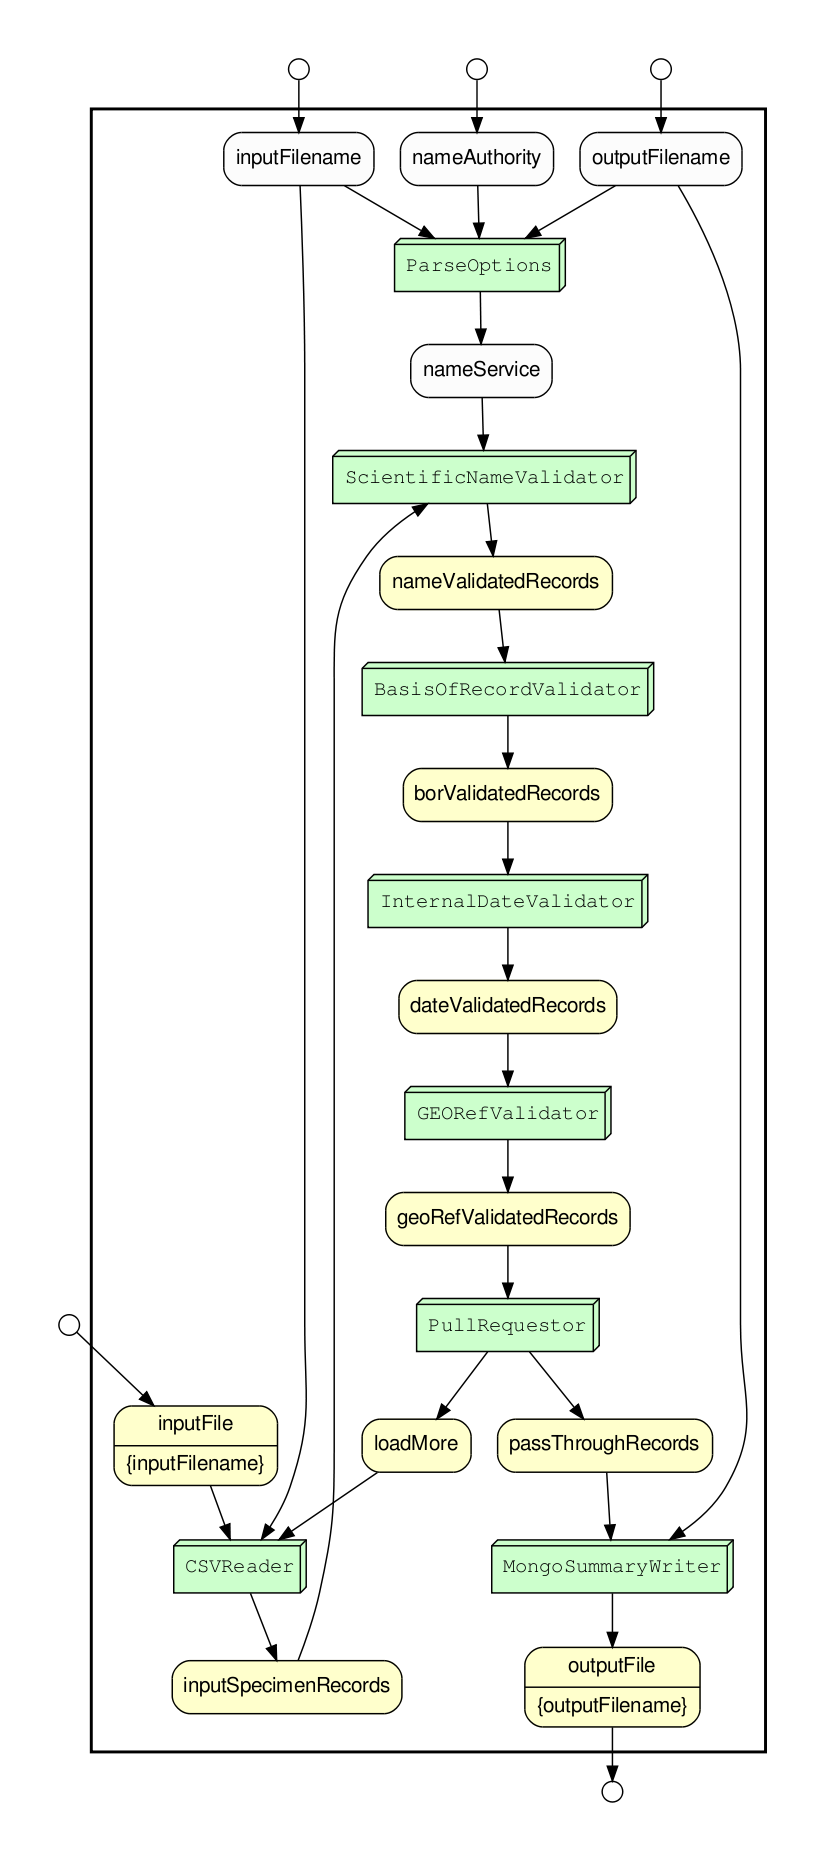
\includegraphics[height=\textheight]{Fig2.png}
\caption{DwCa Workflow}
\label{fig:dwcaWorkflowdia}
\end{figure}

%The para below was moved here in QC34.tex and edited in QC37.tex
Performance testing suggests refactoring our existing actors to be more granular can give us even more of a performance boost, particularly in the case of actors that make calls to external services. The increased granularity allows FP-Akka to assign multiple processors when they are available and also consult a different actor should one block if one of \emph{its} remote services blocks. In addition, increased granularity allows more flexibility in code re\-use.

\section{CSV workflow} \label{CSVWorkflow}

FP-Akka also supports a second use - evaluating and cleaning taxonomic authority tables in natural science collection databases in comparison with external authorities.  FP-Akka-workflowstarter can be invoked using a ``CSV'' workflow with a switch that runs a workflow that includes only a CSV reader, the scientific name validation actor, and a CSV writer.  This workflow is designed to take a dump of data from a taxon authority table, run it against a specified authority, and produce a simple flat report from which records with particular outcomes can be selected to either send to a taxonomically knowlegable collections management staff member to evaluate and correct in the database, or which can be converted (easily with grep/sed/awk) into sql update commands that can be fired against the taxonomic authority table in the database of record.  Figure \ref{fig:largerprocesses} contrasts two ways in which FP-Akka can be incorporated into data quality processes by curators of a natural science collections database of record.


\begin{figure}[h]
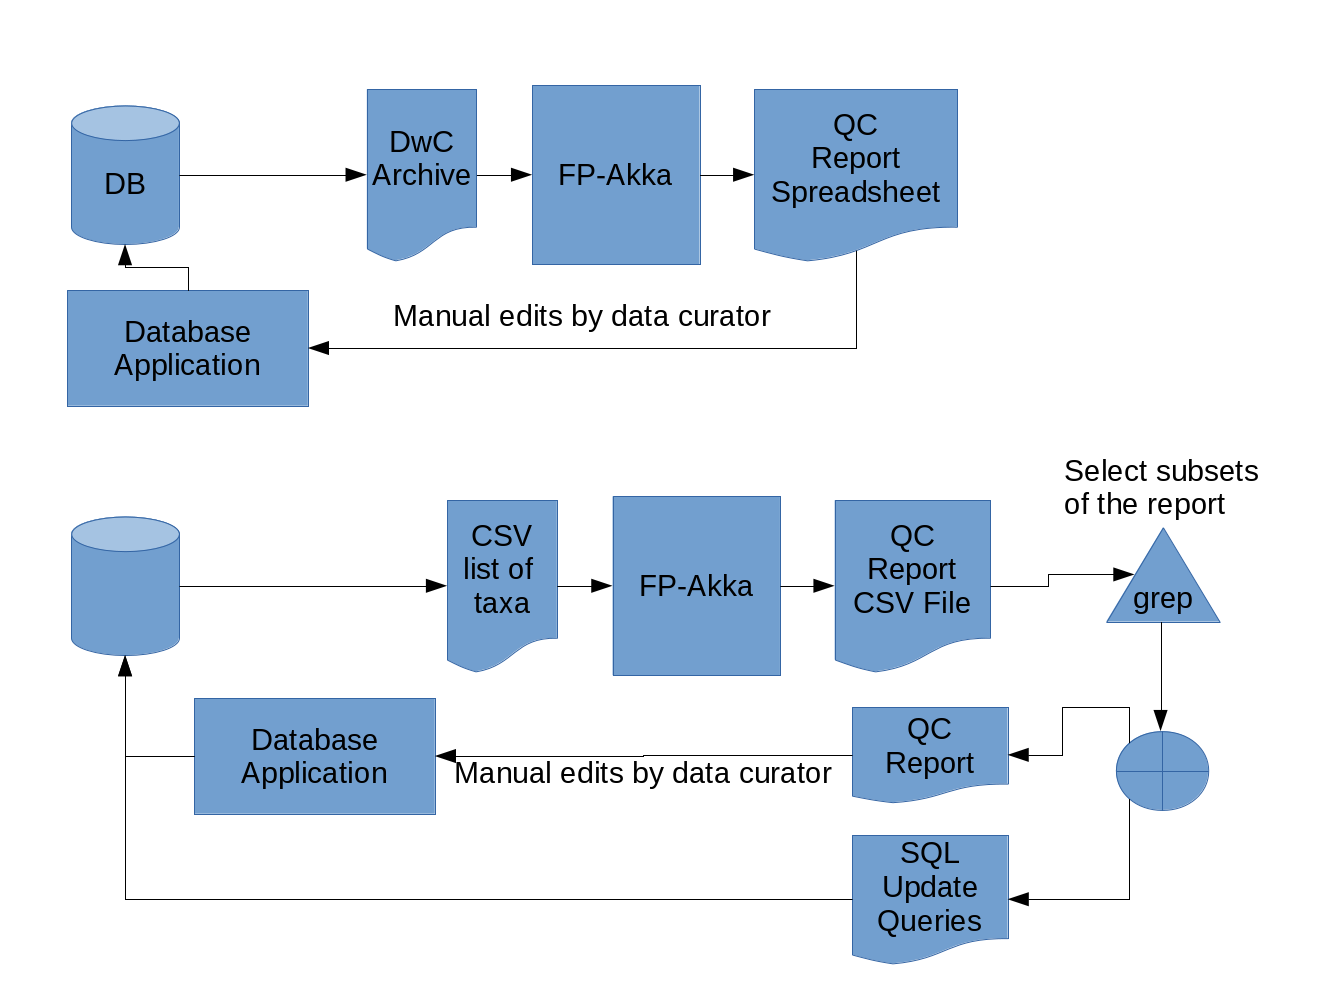
\includegraphics[width=\textwidth]{FP-Akka-externaldataflowpaths.png}
\caption{Incorporation of FP-Akka into data quality procedures in a natural science collection.  Top half of diagram is typical use of the DwCa workflow, bottom half alternative use cases supported by the CSV workflow. Both are described in \citep{Kurator_wiki_2016}}
\label{fig:largerprocesses}
\end{figure}


\section{QC of the QC software}
A QC assertion, especially a systematically occurring one, that is inexplicable to an expert human user may rightly raise the question of whether the input data has exposed a QC issue in the QC software itself. FP-Akka itself is defended in part by standard software engineering QC mechanisms, such as unit testing
\citep{Fraser:2003:DPT:949344.949407} with the JUnit framework \citep{junit-web-2010}, logging application runtime behavior (especially upon timeout of remote services), etc. Some, but not all, of these mechanisms reflect their test results to the console at the time FP-Akka is executed. They are largely targeted at programmers, and their results are not generally available in the post-processor spreadsheet. That kind of QC is outside the scope of this paper.  We have, however, over several years, repeatedly sent the output of FP-akka run on datasets (especially those of the Symbiota Collections of Arthropods Network \citep{SCAN_TCN_website_2016})

%Defects in the software that we have identified through feedback from users of quality control reports include systematic errors (e.g., all marine localities were flagged as errors due to a developer's interpretation of the phrase `on the Earth's surface' to mean on land rather than latitude between +/- 90 degrees), and subtle problems that evaded unit tests, one of which is described below.
Some defects in the software that we have identified through feedback from users of quality control reports include systematic errors. One example was that all marine localities were flagged as errors due to a developer's interpretation of the phrase `on the Earth's surface' to mean on land rather than latitude between +/- 90 degrees.
Some subtle problems evaded unit tests, one of which is described below.
Most of the issues that we are seeing now in feedback from users are yet another class of problem. These are not defects in the software itself, but unexpected values present in the responses from nomenclatural authorities.  For example, in a recent batch of work which involved disambiguating which member of the Sowerby family should be attributed to which scientific names in the taxonomic authority file for Malacology in the Harvard Museum of Comparative Zoology (MCZ), the collection management staff member to whom an FP-Akka report was given noted that the authorship for the genus Stilifer of `Broderip [in Broderip \& Sowerby I], 1832' seemed odd.  FP-Akka, consulting WoRMS, had taken the input dwc:scientificName=Stilifer, dwc:scientificNameAuthorship=Broderip and Sowerby, 1832, had returned the record as curated, with the curation comment ``Found plausible match in WoRMS: Specifying Which Sowerby, Year Exact'' and a guid for the match in WoRMS of urn:lsid:marinespecies.org:taxname:205197.  The user was expecting, for their purpose, for the formulation of the correction to be Stilifer Broderip and Sowerby, 1832 curated as Stilifer Broderip, 1832, instead of the formulation presented by WoRMS.  We have seen similar issues in other zoological authorities, where the facts presented from the authority are correct, but the format presented from the authority does not match the expectations of the user of the FP-Akka report.\footnote{See http://marinespecies.org/aphia.php?p=taxdetails\&id=205197}

We next describe serious misbehavior of FP-Akka in response to curious, surely unintended, georeference, in the data described in 
the DwC Archive served by \citep{SpiderDiversityCorrigendum2015} as of November 12, 2015. 
The occurrence data in that DwCa had all decimalLatitude and decimalLongitude 10 times the intended values, e.g. latitude 458.797 (rather than 45.87556) and longitude 139.468 (rather than 13.948889) for the Slovenian town of Budanje.  One of the georeference errors for which FP-Akka checks is an off by a factor of ten error in decimal latitude and longitude values.  The expected response for these input values would be either curation to the divided by 10 values, or a marker that the record was in error.  In many cases, however, FP-Akka asserted that these numerically invalid input values were correct, with provenance suggesting that the widely used Tulane Geolocate service was accepting such values and---inspection showed---was querying and getting answers for values as though divided by 10.  For the example, the FP-Akka output signaled ``no change needed'' for what is clearly a ridiculous result. However, in this case, the spreadsheet provenance column carried the text 

``\sffamily found 1 possible georeferences with Geolocate engine:GLC:4.95\textbar U:1.01374\textbar eng:1.0 \textbar BUDANJE score:82 45.875556 13.948889 km:0 \textbar Original coordinates are near (within georeference error radius or 20.0 km) the georeference for the locality text from the Geolocate service.  Accepting the original coordinates.\rmfamily'' 

This suggested erroneously that the original coordinates are acceptable, while at the same time indicating that the Geolocate service, invoked with locality Budanje, returned reasonable coordinates. 


Investigation of our georeference validation code located a subtle defect in a method that finds the distance between two points on the earth independent of latitude, and a unit test that was correct, but of inadequate scope to catch this defect.  Examination of the code revealed two places at which the invocation of the trigonometric functions $sin$ and $cos$ neglected to convert latitude and longitude to radians as assumed by the Java Math library. Consider comparing the points $(458.797,139.468)$ and $(45.87556, 13.9468)$ 
%(\textbf{Discuss further?, i.e. exactly when. Bob says no--it's too diversionary}
%Under some circumstances the spherical trigonometry function $haversine$ a factor containing the erroneous
For the first of these points, the spherical trigonometry function $haversine$ has a factor containing the erroneous
$cos(458.797)$ hence was driven negative and so was the term containing that factor. To get a great circle distance in km between the two points, this term is fed to the square root function $sqrt$ thence to the arctangent function $atan2$ with corresponding erroneous longitude. But the square root of a negative number is not a real number, so $sqrt$ returns the Java numeric constant NaN (``Not a Number'').  Subsquently NaN is passed to $atan2$ which returns $0$ on these NaN's to compute the great circle distance.  Thus  $(458.797,139.468)$ and $(45.87556, 13.9468)$ are the same point in the face of our coding error.  The unit test asked the method to calculate the distance from the equator to 1 degree North, and the distance from one point on the equator to one degree West of that point.  In both cases, a zero value was passed in to be multiplied by the results of the sine and cosine functions that were handed degrees instead of radians, causing the error to go away and for these narrow cases, for a correct result to be returned.  A unit test (now present) that asked for the distance between two arbitrary points on the surface of the earth, neither on the equator or Greenwich meridian, would have failed.  Thus, the issue had nothing to do with the Geolocate service. The current release of FP-Akka has correct code.

A key point in this realization of where defects may lie is expectation management for the end users - things we report as errors may be defects in their data, defects in our code, or defects in the authorities our workflows are consulting.  Users to whom the data quality report is presented without this understanding may observe what they percieve as errors in the data quality report. They might dismiss the reporting framework as defective, unless they understand that their data may expose errors in the framework that the developers can readily fix, or that the errors are in the external authoritative sources that the software consulted.  
\section{Acknowledgements}
The SCAN curators and participants in Kurator workshops who have reviewed FP-Akka QC reports on their data.  
Brendan Haley and Adam Baldinger in the MCZ who have reviewed FP-Akka QC reports on their data.
Susan Morris for comments on the manuscript.


%\section{Figures}
\begin{appendices}
\section{MCZData}
\begin{quote}https://github.com/kurator-org/FP-Akka-Manuscript/blob/master/data\_in\_and\_data\_out\_v2.xls\end{quote}
\section{Another}
\appendix
\newpage
\begin{center}
\Huge{Appendices}
\end{center}
\textbf{As long as this note is here, the appendices details are likely to change radically, so while comments are welcome, I recommend just read for the gist....Bob}

Likely appendences:

- small postprocess xls output limited to about 5 rows covering the examples discussed in Table  \ref{ExampleQCAssertions}

\begin{lstlisting}
\end{lstlisting}

\end{appendices}

\newpage
\bibliography{bib1}{}
\end{document}
